%
% This template has been downloaded from:
% http://www.LaTeXTemplates.com
%
%
%%%%%%%%%%%%%%%%%%%%%%%%%%%%%%%%%%%%%%%%%

%----------------------------------------------------------------------------------------
%	PACKAGES AND THEMES
%----------------------------------------------------------------------------------------

\documentclass{beamer}

\mode<presentation> {

% The Beamer class comes with a number of default slide themes
% which change the colors and layouts of slides. Below this is a list
% of all the themes, uncomment each in turn to see what they look like.

%\usetheme{default}
%\usetheme{AnnArbor}
%\usetheme{Antibes}
%\usetheme{Bergen}
%\usetheme{Berkeley}
%\usetheme{Berlin}
%\usetheme{Boadilla}
%\usetheme{CambridgeUS}
\usetheme{Copenhagen}
%\usetheme{Darmstadt}
%\usetheme{Dresden}
%\usetheme{Frankfurt}
%\usetheme{Goettingen}
%\usetheme{Hannover}
%\usetheme{Ilmenau}
%\usetheme{JuanLesPins}
%\usetheme{Luebeck}
%\usetheme{Madrid}
%\usetheme{Malmoe}
%\usetheme{Marburg}
%\usetheme{Montpellier}
%\usetheme{PaloAlto}
%\usetheme{Pittsburgh}
%\usetheme{Rochester}
%\usetheme{Singapore}
%\usetheme{Szeged}
%\usetheme{Warsaw}

% As well as themes, the Beamer class has a number of color themes
% for any slide theme. Uncomment each of these in turn to see how it
% changes the colors of your current slide theme.

%\usecolortheme{albatross}
%\usecolortheme{beaver}
%\usecolortheme{beetle}
%\usecolortheme{crane}
%\usecolortheme{dolphin}
%\usecolortheme{dove}
%\usecolortheme{fly}
%\usecolortheme{lily}
%\usecolortheme{orchid}
%\usecolortheme{rose}
%\usecolortheme{seagull}
%\usecolortheme{seahorse}
%\usecolortheme{whale}
%\usecolortheme{wolverine}

%\setbeamertemplate{footline} % To remove the footer line in all slides uncomment this line
%\setbeamertemplate{footline}[page number] % To replace the footer line in all slides with a simple slide count uncomment this line

%\setbeamertemplate{navigation symbols}{} % To remove the navigation symbols from the bottom of all slides uncomment this line
}

\usepackage{graphicx} % Allows including images
\usepackage{booktabs} % Allows the use of \toprule, \midrule and \bottomrule in tables
%\usepackage[normalem]{ulem}
\usepackage{cancel}

%----------------------------------------------------------------------------------------
%	TITLE PAGE
%----------------------------------------------------------------------------------------

\title[The Power of Actors]{The Power of \cancel{LOVE}... Actors} % The short title appears at the bottom of every slide, the full title is only on the title page

\author{Bernhard St\"ocker} % Your name
\institute[UCLA] % Your institution as it will appear on the bottom of every slide, may be shorthand to save space
{
Recogizer Group GmbH\\ % Your institution for the title page
\medskip
\textit{bernhard.stoecker@recogizer.de} % Your email address
}
\date{\today} % Date, can be changed to a custom date

\begin{document}

\begin{frame}
\titlepage % Print the title page as the first slide
\end{frame}

\begin{frame}
\frametitle{Overview} % Table of contents slide, comment this block out to remove it
\tableofcontents % Throughout your presentation, if you choose to use \section{} and \subsection{} commands, these will automatically be printed on this slide as an overview of your presentation
\end{frame}

%----------------------------------------------------------------------------------------
%	PRESENTATION SLIDES
%----------------------------------------------------------------------------------------

%------------------------------------------------
\section{What are Actors?} % Sections can be created in order to organize your presentation into discrete blocks, all sections and subsections are automatically printed in the table of contents as an overview of the talk
%------------------------------------------------

%\subsection{Subsection Example} % A subsection can be created just before a set of slides with a common theme to further break down your presentation into chunks

\begin{frame}
\frametitle{What are Actors?}
\Huge{\centerline{What are Actors?}}
\end{frame}

%------------------------------------------------

\begin{frame}
\frametitle{What are Actors?}
Act-or: to act: \textbf{\emph{"to do something for a particular purpose or to solve a problem"}} (From the Cambridge dictionary)
\end{frame}

%------------------------------------------------

\begin{frame}
\frametitle{What are Actors?}
Wikipedia:
\begin{itemize}
\item A mathematical model of concurrent computation
\item Actors can hold and modify private state
\item Affect each other through messages only
\item In response to a message that it receives, an actor can:
\begin{itemize}
\item Make local decisions
\item Create more actors
\item Send more messages
\item Respond to the incoming message
\end{itemize}
\end{itemize}
\end{frame}

%------------------------------------------------

\section{WhatsApp}

\begin{frame}
\frametitle{WhatsApp}
\Huge{\centerline{WhatsApp}}
\end{frame}


%------------------------------------------------

\begin{frame}
\frametitle{WhatsApp???}

\includegraphics[width=0.8\linewidth]{./whatsup.jpg}
\end{frame}

%------------------------------------------------

\begin{frame}
\frametitle{WhatsApp}
\begin{itemize}
\item Every user has an actor representing her
\item When sending a message my actor sends a message to all related users
\item The users receiving a message ensure the message is delivered.
\end{itemize}
\end{frame}

%------------------------------------------------

\begin{frame}
\frametitle{WhatsApp}
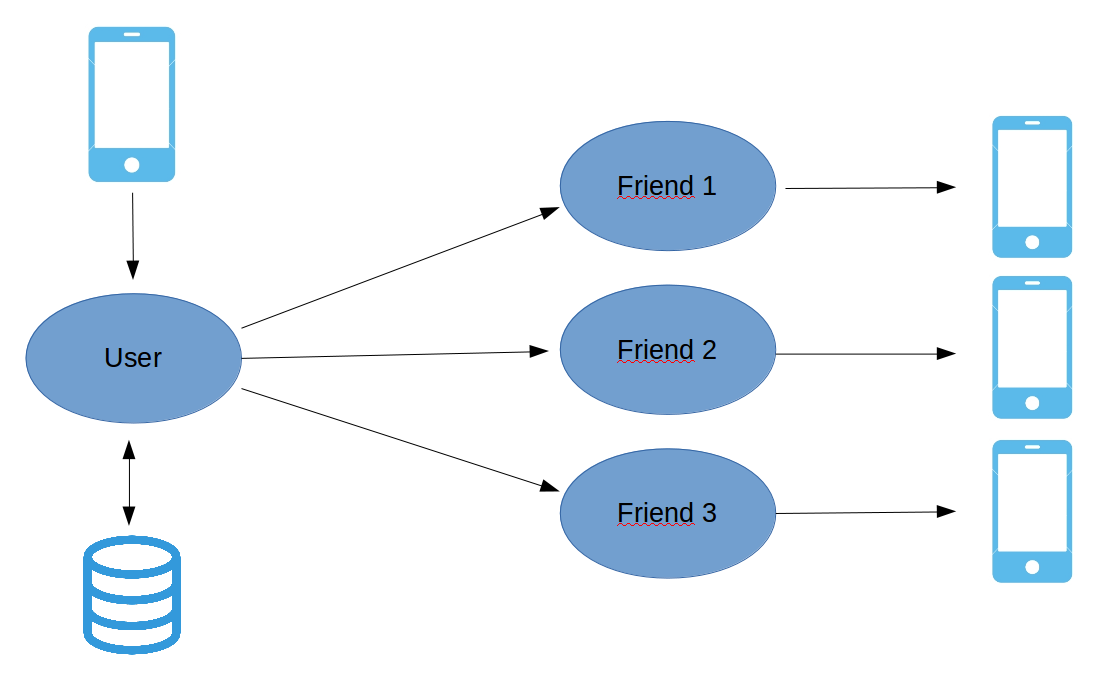
\includegraphics[width=0.95\linewidth]{./whatsapp_actor.png}
\end{frame}

%------------------------------------------------

\section{Actors in Elixir}

\begin{frame}
\frametitle{Actors in Elixir}
\Huge{\centerline{Actors in Elixir}}
\end{frame}

%------------------------------------------------

\begin{frame}
\frametitle{Actors in Elixir}
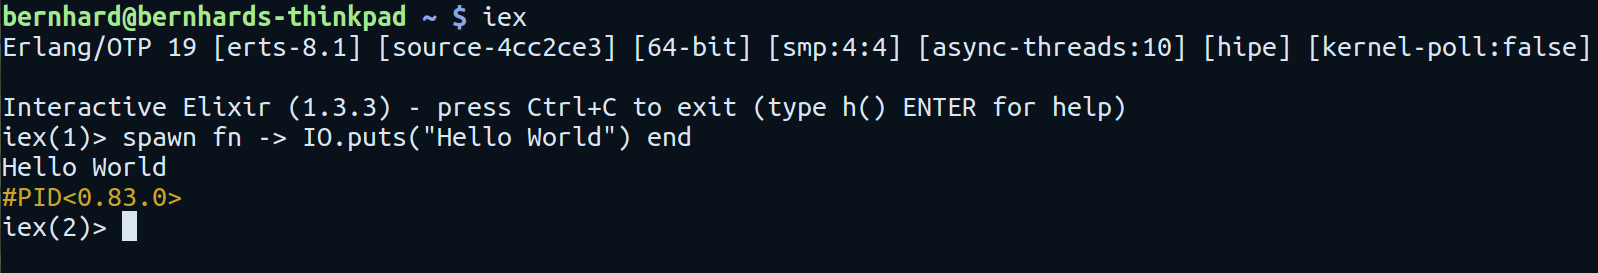
\includegraphics[width=1.2\linewidth]{./hello_elixir.jpg}
\end{frame}

%------------------------------------------------

\begin{frame}
\frametitle{Actors in Elixir}
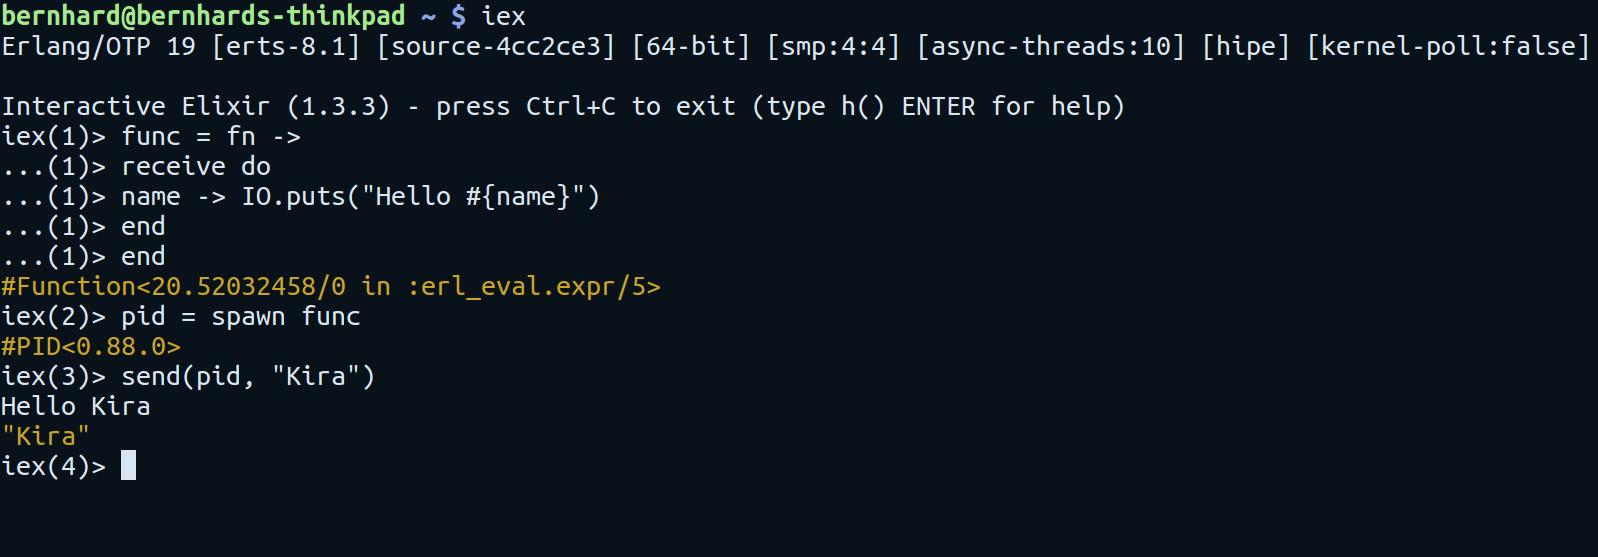
\includegraphics[width=1.2\linewidth]{./elixir_hello_kira.jpg}
\end{frame}


\begin{frame}
\frametitle{Actors in Elixir}
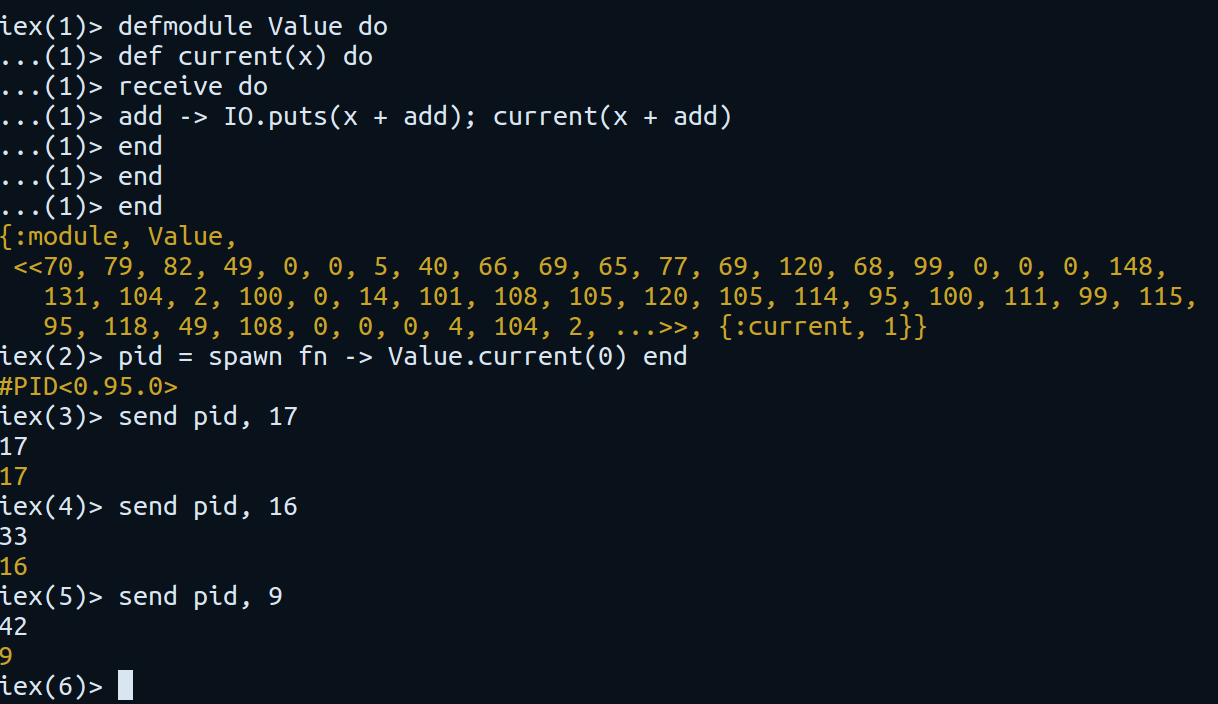
\includegraphics[width=1.15\linewidth]{./elixir_state.png}
\end{frame}

%------------------------------------------------

\begin{frame}
\frametitle{Actors in Elixir}
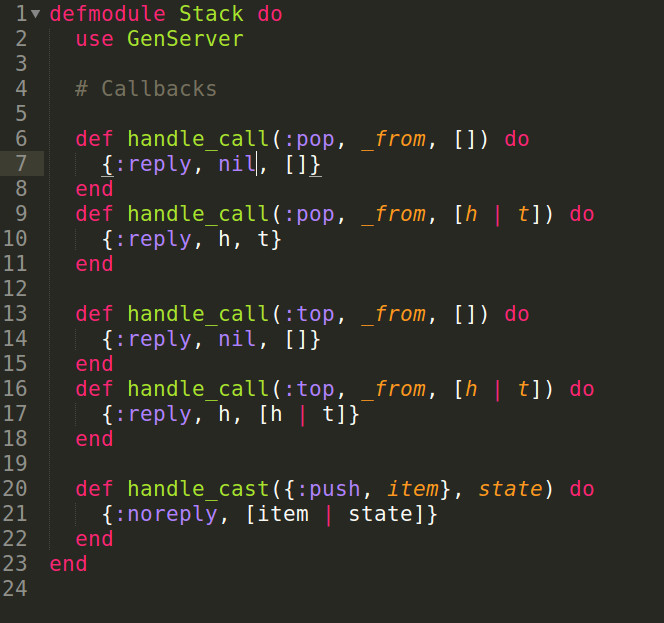
\includegraphics[width=0.6\linewidth]{./GenServerCode.jpg}
\end{frame}

%------------------------------------------------

\begin{frame}
\frametitle{Actors in Elixir}
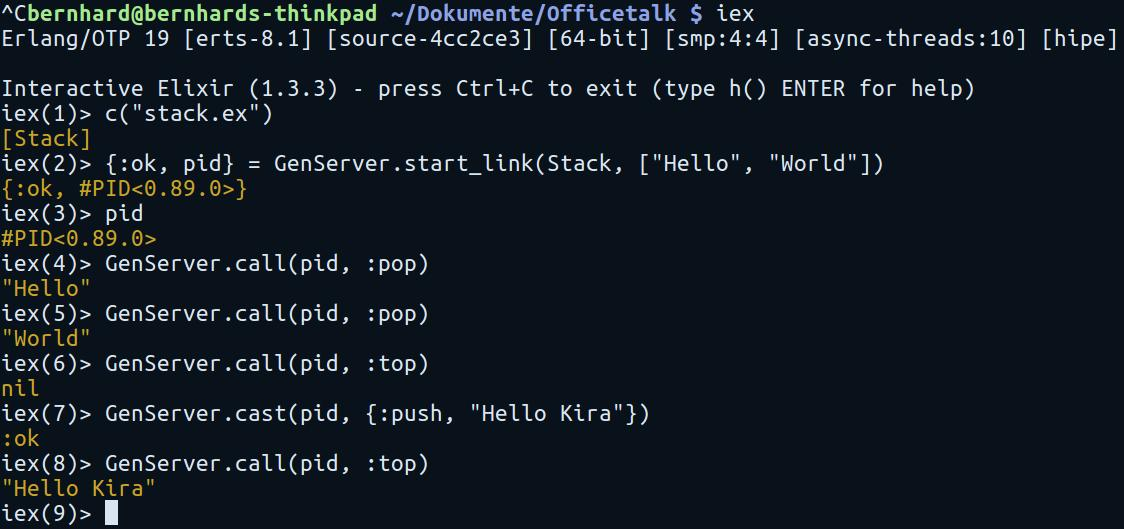
\includegraphics[width=1.25\linewidth]{./GenServerTerminal.jpg}
\end{frame}

%------------------------------------------------

\section{Actors in Scala}

\begin{frame}
\frametitle{Actors in Scala}
\Huge{\centerline{Actors in Scala}}
\end{frame}


%------------------------------------------------

\begin{frame}
\frametitle{Actors in Scala}
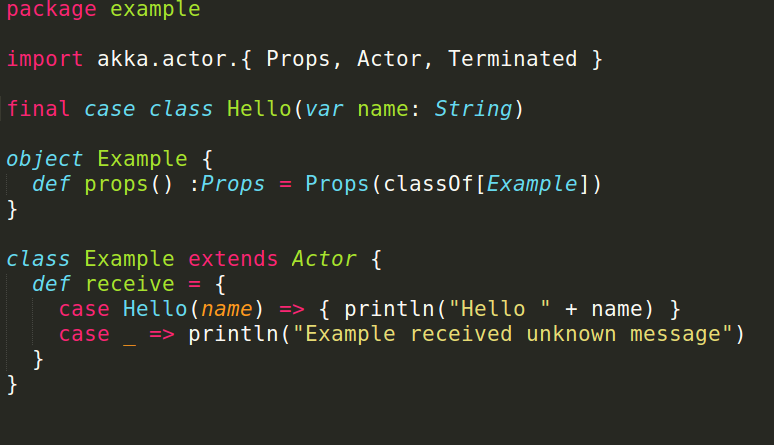
\includegraphics[width=1\linewidth]{./scala_example_actor.png}
\end{frame}

%------------------------------------------------

\begin{frame}
\frametitle{Actors in Scala}
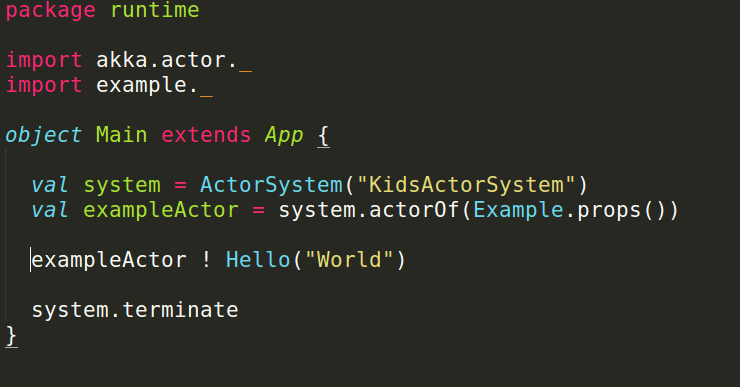
\includegraphics[width=1\linewidth]{./scala_example_main.png}
\end{frame}

%------------------------------------------------

\begin{frame}
\frametitle{Actors in Scala}
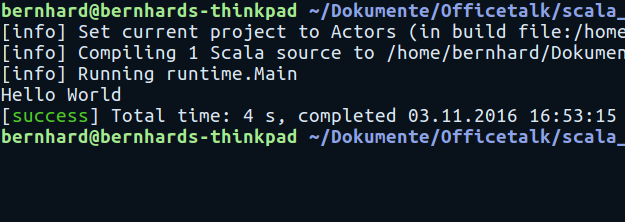
\includegraphics[width=1\linewidth]{./scala_example_terminal.png}
\end{frame}

%------------------------------------------------

\begin{frame}
\frametitle{Actors in Scala}
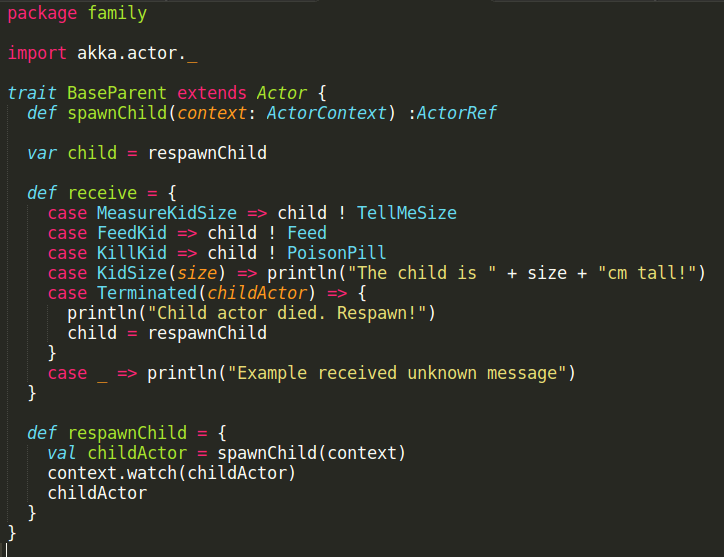
\includegraphics[width=0.8\linewidth]{./parent_trait.png}
\end{frame}

%------------------------------------------------

\begin{frame}
\frametitle{Actors in Scala}
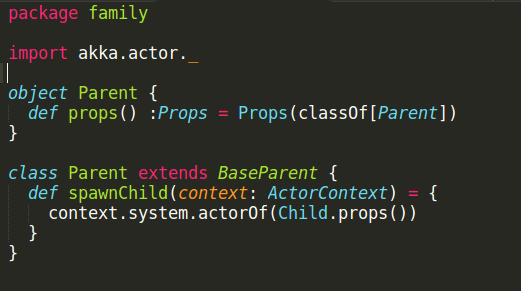
\includegraphics[width=0.8\linewidth]{./parent_actor.png}
\end{frame}

%------------------------------------------------

\begin{frame}
\frametitle{Actors in Scala}
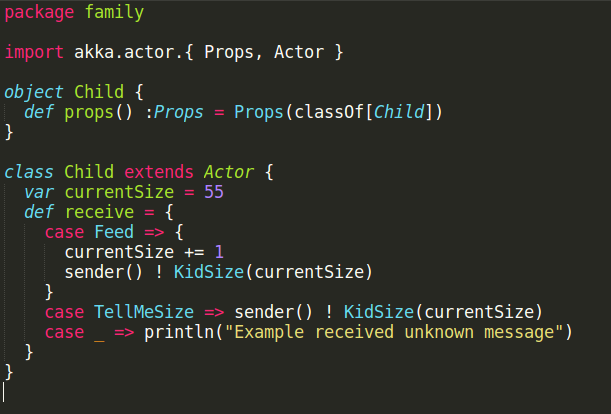
\includegraphics[width=0.9\linewidth]{./parent_child.png}
\end{frame}

%------------------------------------------------

\begin{frame}
\frametitle{Actors in Scala}
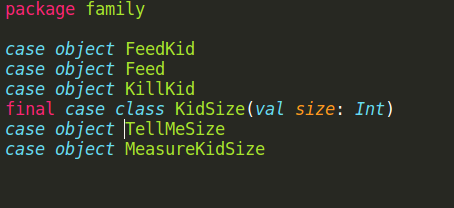
\includegraphics[width=1\linewidth]{./parent_messages.png}
\end{frame}

%------------------------------------------------

\begin{frame}
\frametitle{Actors in Scala}
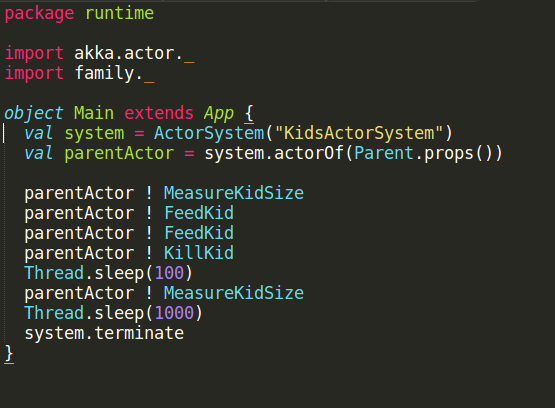
\includegraphics[width=0.8\linewidth]{./parent_main.png}
\end{frame}

%------------------------------------------------

%TODO some refs
%------------------------------------------------

\begin{frame}
\Huge{\centerline{The End}}
\end{frame}

%----------------------------------------------------------------------------------------

\end{document} 